\documentclass[11pt]{article}
\usepackage[a4paper, top=2.5cm, bottom=2.5cm, left=2.5cm, right=2.5cm]{geometry}
\usepackage{amsmath, amssymb}
\usepackage{xcolor}
\usepackage{tikz}
\usetikzlibrary{arrows.meta}
\definecolor{tdc1}{HTML}{A05A5A}
\definecolor{tdc2}{HTML}{E53935}
\definecolor{tdc3}{HTML}{7E57C2}

\title{Electrostatics (sample)}
\date{}

\begin{document}
\maketitle

\begin{center}
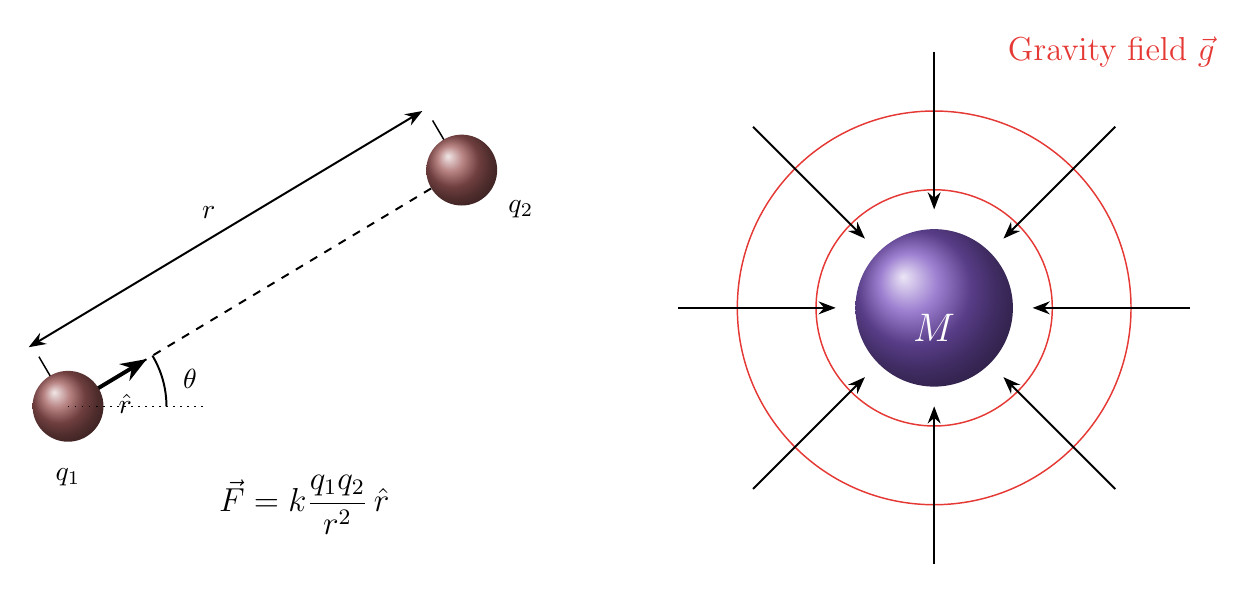
\begin{tikzpicture}[x=1cm, y=1cm]
  % diagramtex-data: …
  \draw[line width=0.71pt, dashed] (1,-5) -- (6,-2);
  \draw[line width=0.71pt, {Stealth}-{Stealth}] (0.5,-4.25) -- node[auto, pos=0.5] {$r$} (5.5,-1.25);
  \draw[line width=0.53pt] (1,-5) -- (0.63,-4.37);
  \draw[line width=0.53pt] (6,-2) -- (5.63,-1.37);
  \draw[line width=1.42pt, -{Stealth}] (1,-5) -- node[auto, swap, pos=0.5] {$\hat{r}$} (2,-4.4);
  \shade[ball color=tdc1] (1,-5) circle (0.45);
  \shade[ball color=tdc1] (6,-2) circle (0.45);
  \node at (1,-5.9) {$q_1$};
  \node at (6.75,-2.5) {$q_2$};
  \node[font=\large] at (4,-6.25) {$\vec F = k\dfrac{q_1 q_2}{r^2}\,\hat r$};
  \draw[draw=tdc2, line width=0.53pt] (12,-3.75) circle (1.5);
  \draw[draw=tdc2, line width=0.53pt] (12,-3.75) circle (2.5);
  \draw[line width=0.71pt, -{Stealth}] (15.25,-3.75) -- (13.25,-3.75);
  \draw[line width=0.71pt, -{Stealth}] (14.3,-6.05) -- (12.88,-4.63);
  \draw[line width=0.71pt, -{Stealth}] (12,-7) -- (12,-5);
  \draw[line width=0.71pt, -{Stealth}] (9.7,-6.05) -- (11.12,-4.63);
  \draw[line width=0.71pt, -{Stealth}] (8.75,-3.75) -- (10.75,-3.75);
  \draw[line width=0.71pt, -{Stealth}] (9.7,-1.45) -- (11.12,-2.87);
  \draw[line width=0.71pt, -{Stealth}] (12,-0.5) -- (12,-2.5);
  \draw[line width=0.71pt, -{Stealth}] (14.3,-1.45) -- (12.88,-2.87);
  \shade[ball color=tdc3] (12,-3.75) circle (1);
  \node[font=\Large, text=white] at (12,-4) {$M$};
  \node[font=\large, text=tdc2] at (14.25,-0.5) {Gravity field $\vec g$};
  \draw[line width=0.71pt] (2.25,-5) arc[start angle=0, end angle=31, radius=1.25];
  \draw[line width=0.53pt, dotted] (1,-5) -- (2.75,-5);
  \node at (2.55,-4.65) {$\theta$};
\end{tikzpicture}
\end{center}

\end{document}
